\chapter{Introduction}
\label{ch:introduction}

\section{Preface}

\co{Different phases of matter exist and are determined by the way the atoms are organized.}
Even though all matter consists of atoms, it can appear in various forms and have various properties.
Familiar examples include solids, gases, and liquids; however, more exotic forms exist, such as superfluids, magnets, plasmas, and Bose-Einstein condensates.
These different forms of matter are called phases or states of matter.
The various properties of materials arise from the different phases (ways atoms structure itself in a material).

\co{Symmetry-breaking theory explains how to understand the different phases of matter.}
Symmetry-breaking theory provides a way to understand many of the different phases.
It explains that these different phases correspond to different symmetries in the way the atoms are structured.
Whenever the phase of a material changes (called a phase transition), the symmetry of the organization of the atoms changes.
For example, in a liquid, the atoms are distributed randomly, when moving the atoms by an arbitrary distance it stays a liquid.
This property indicates that a liquid has a continuous translation symmetry.
When a liquid goes through a phase transition and turns into a crystal (e.g.~water to ice), the atoms organize into a lattice.
Only when moving the atoms by an exact integer number of the lattice constant (the distance between the smallest repeating pattern), the crystal remains the same.
This property indicates that a crystal has a discrete translation symmetry.
This phase transition is an example of symmetry breaking because it reduces the continuous translation symmetry of the liquid to the discrete symmetry of the crystal.
Another example is ferromagnets, where the spins of electrons are randomly oriented above a certain critical temperature $T_\textrm{c}$: having a continuous rotational symmetry.
However, when $T<T_\textrm{c}$ the spin align: resulting in a discrete rotational symmetry.

\co{Symmetry-breaking theory works well but not for topologically ordered matter.}
This symmetry-breaking theory was introduced by Lev Landau in 1937~\cite{Landau1937}.
It was long believed that it explains all phases in materials and all (continuous) phase transitions.
In 1987, in an attempt to describe high $T_\textrm{c}$ superconductors, the chiral spin state was introduced~\cite{Kalmeyer1987}.
However, it was soon realized that the symmetry breaking description was not sufficient to explain its phase.
A new kind of phase called a ``topological phase'' was introduced~\cite{Wen1989,XiaoGang1990}.
It is a zero-temperature phase of matter (i.e.~quantum matter) that is described by a robust ground state degeneracy.
This degenerate ground state has quantized non-Abelian geometric phases; we discuss what this means in Sec.~\ref{sec:braiding}.

\co{The QHE is an example that can be described using of the theory of topological order.}
The quantum Hall effect is an example of a state that cannot be described by its symmetries alone. Instead, it can be characterized by a distinct topology (see Fig.~\ref{fig:knots})~\cite{Avron2003}.
Its signature, shown in Fig.~\ref{fig:qhe}, is robust and does not depend on the specific geometry and does not vanish upon smooth changes in the material's parameters.
Its signature is an exact quantization of the Hall conductance of an integer number of $e^2/h$, where $e$ is the elementary charge, and $h$ is the Planck constant, both fundamental constants.
Because of its robustness---it is insensitive to specific experimental settings and purity of the material used---the quantum Hall effect is used to determine the standard for electrical resistance\cite{Jeckelmann2001}.
The effect appears upon applying a large perpendicular magnetic field $B_\perp$ to a two-dimensional electron gas at low temperatures.
This opens a gap between the energy bands and localizes the electrons in the bulk.
Classically, we can visualize what happens, as electrons localizing in small cyclotron orbits; this leaves the electrons near the edges of the material to bounce along the edges.
These states that propogate along the edges are responsible for the conduction and are called ``edge states.''

\begin{figure}[!htb]
\begin{center}
% \includegraphics{chapter_introduction/figures/knots.pdf}  % XXX: add this figure
\caption{
Topology in mathematics studies the properties of an object that are preserved under continuous deformations.
For example, an unknot (left) cannot be continuously transformed into a trefoil knot (right) without cutting it; this means that they are not topologically equivalent.
The object that is studied in condensed matter physics, is the Hamiltonian.
Two Hamiltonians are topologically equivalent whenever an Hamiltonian can be continuously transformed into another Hamiltonian.
Unlike a knot that can be visualized in space, the topology of the quantum Hall state manifests itself in momentum space.
\label{fig:knots}}
\end{center}
\end{figure}

\begin{figure}[!htb]
\begin{center}
% 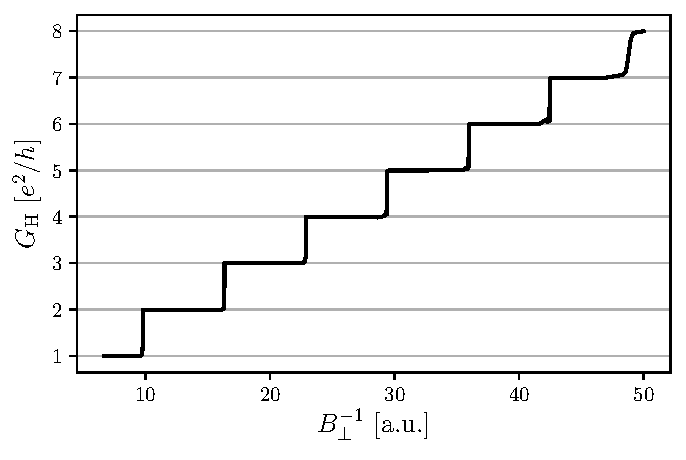
\includegraphics{chapter_introduction/figures/qhe.pdf}  % XXX: add this figure
\caption{
The integer quantum Hall effect.
The Hall resistance $R_H$ (reciprocal of the Hall conductance $G_H$) of a two-dimensional electron gas as a function of the perpendicular magnetic field $B_\perp$ at low-temperature.
It displays a stairlike quantized sequence of Hall conductances equal to $ne^2/h$, where $n$ is an integer characterizing each plateau.
\label{fig:qhe_example}}
\end{center}
\end{figure}

\co{More topological states have been realized, one example is TIs.}
The field of topology in condensed matter has substantially grown over the past decades.
Recently, in 2016, the Nobel prize was awarded to Thouless, Haldane, and Kosterlitz for the theoretical findings of topological states.
One of these new states are ``topological insulators,'' which also exhibit edge or surface states and have similarities to the quantum Hall effect, but do not require extreme conditions such as the large magnetic field.
Here, spin-orbit coupling replaces the effect of the magnetic field.
This is a coupling between the electron's momentum and spin, effectively causing a momentum dependent magnetic field for electrons that move through a crystal lattice.
The spin-orbit coupling effect is discussed in more detail in Sec.~\ref{sec:hamiltonian_term_by_term}.
Due to the absence of a magnetic field (which breaks time-reversal symmetry in the quantum Hall effect), the edge states always come in counter-propagating pairs, shown in see Fig.~\ref{fig:qhe_example}.

\begin{figure}[!htb]
\begin{center}
% \includegraphics{chapter_introduction/figures/qhe_vs_ti.pdf}
\caption{
Comparison of an insulator, quantum Hall effect, and a topological insulator.
% XXX: Rip Fig. 2 and 5 from 10.1103/RevModPhys.82.3045
\label{fig:qhe}}
\end{center}
\end{figure}

\co{Topological states might be used to build a topological quantum computer.}
Besides the exciting new fundamental physical insights into topological materials, topological states might be used to design novel new quantum devices.
One of the most exciting applications of topological states, is to use them to build a topological quantum computer by exploiting their non-Abelian properties.
It is predicted that a quantum computer is much faster than a classical computer in performing certain tasks.
For example, the simulation of quantum systems~\cite{Feynman1982} and prime factorization~\cite{Shor1994}.
The fundamental building block of the quantum computer is the qubit (or quantum bit), which is the quantum equivalent of the classical transistor.
Because these qubits store quantum information, they are extremely fragile, and even a small interaction with its environment can destroy its state, which results in computational errors.
Physicists experiment with different approaches to create a qubit; for example, there are proposals (and some realizations of) qubits based on quantum optics~\cite{Kok2007}, ultracold atoms~\cite{Friis2018}, spin-based systems~\cite{Vandersypen2017}, and superconducting systems~\cite{Arute2019}.
In general, one of the most significant problems is to limit and correct the computational errors, and therefore a large fraction of the research is focussed on error-correction~\cite{Lidar2013}.
Here, the advantage of using topological states becomes apparent because the topological qubit naturally protects its state against small perturbations in the environment~\cite{Nayak2008}.

\co{Majoranas can be used to create this topological quantum computer.}  % XXX: maybe mention that Majoranas are topologically protected
The zero-energy Majorana bound state (MBS) is the simplest non-Abelian excitation.
The MBS was first proposed to exist as quasiparticle excitations of the $\nu = 5/2$ quantum Hall effect~\cite{Read2000,Moore1991}, which requires a high material quality and very low temperatures.
Other early proposals~\cite{Gurarie2005,Sarma2006,Tewari2007} rely on rare and exotic $p$-wave superconductors and are extremely challenging to realize experimentally.
In 2008, Fu and Kane suggested a new approach to create MBSs by using a hybrid structure of an ordinary $s$-wave superconductor coupled to a topological insulator to create a state that resembles a spinless $p$-wave superconductor~\cite{Fu2008}.
Inspired by this hybrid approach, in 2010, two works~\cite{Lutchyn2010,Oreg2010} suggested using a simpler one-dimensional nanowire system coupled to a $s$-wave superconductor.
This simple model combines spin-orbit coupling, superconductivity, electrostatic tunability, and an applied magnetic field.
When tuned into the right parameter regime, this system hosts MBSs at the edges of the nanowire.
Since its introduction, many experiments have detected signatures of MBSs~\cite{Mourik2012,Das2012,Deng2012,Deng2016,Deng2016a,Chen2017a}; however, none have demonstrated the presence of MBSs with absolute certainty by showing its non-Abelian statistics.
Because of the simplicity of the model, it can be solved analytically; however, it neglects many physical phenomena that are crucial for understanding the properties of the MBSs.

\co{In this thesis, we study the hybrid Majorana model.}
In this thesis, we study extensions to this model and go beyond the regime that can be studied analytically.
The next sections introduce superconductivity and the topological protection of Majoranas (Sec.~\ref{sec:superconductivity}), non-Abelian statistics (Sec.~\ref{sec:braiding}), the minimal hybrid Majorana model (Sec.~\ref{sec:minimal_majoranas}), and finally, a few extensions to this model (Sec.~\ref{sec:realistic_nanowire}).
At that point, it should be evident that solving this problem requires numerical methods, which is the topic of Sec.~\ref{sec:numerical_methods}.


%%%%%%%%%%%%%%%%%%%%%%%%%%%%%%%%%%%%%%%%%%%%%%%%%%%%%%%%%%%%%%%%%%%%%%%%%%%%%%%%%%%%%%%
%%%%%%%%%%%%%%%%%%%%%%%%%%%%%%%%%% SUPERCONDUCTIVITY %%%%%%%%%%%%%%%%%%%%%%%%%%%%%%%%%%
%%%%%%%%%%%%%%%%%%%%%%%%%%%%%%%%%%%%%%%%%%%%%%%%%%%%%%%%%%%%%%%%%%%%%%%%%%%%%%%%%%%%%%%


\section{Topological protection of Majoranas}\label{sec:superconductivity}
\co{To understand the topological protection of MBS in hybrid structures, we discuss superconductivity.}
This section discusses superconductivity to understand the topological protection of Majorana bound states.
Superconductivity is a phenomenon that occurs in certain materials.
These materials become superconducting when they are cooled below a characteristic critical temperature $T_{\mathrm{c}}$.
Upon reaching this temperature, the material undergoes a phase transition that results in precisely zero electrical resistance and the expulsion of magnetic fields.
Superconductivity was discovered by Heike Kamerlingh Onnes in 1911, and ever since, considerable efforts have been devoted to finding out how and why it works.
The phenomenological Ginzburg-Landau theory and the microscopic BCS theory led to a good understanding of ``conventional'' superconductivity.
A lot of today's research focuses on exotic superconductors, high $T_{\mathrm{c}}$ superconductors, and hybrid structures that consist of a superconductor and another material.
In this thesis, we study such hybrid structures.

\subsection{BCS theory and the mean-field approximation}\label{sec:BCS-theory}
\co{We can model superconductivity using BCS theory.}
BCS theory describes superconductivity as a microscopic effect.
It assumes that two electrons from a Cooper pair of two electrons, where the electrons effectively attract due to electron-phonon coupling~\cite{Cooper1956,Bardeen1957,Bardeen1957a}.
It postulates that superconductivity is caused by a condensation of these Cooper pairs at the Fermi energy\footnote{We assume zero temperature $\left(T=0\right)$, so $E_{\textrm{F}}=\mu$, where $\mu$ is the chemical potential.} $E_{\textrm{F}}$ into a boson-like state, a Bose Einstein condensate.
The model Hamiltonian in the language of second quantization ~\cite{Gennes1999} is
\begin{equation}
\mathcal{H}_{\textrm{BCS}}=\sum_{\bm{k}\sigma}\epsilon_{\bm{k}}c_{\bm{k}\sigma}^{\dagger}c_{\bm{k}\sigma}+\sum_{\bm{k}\bm{l}}V_{\bm{k}\bm{l}}c_{\bm{k}\uparrow}^{\dagger}c_{-\bm{k}\downarrow}^{\dagger}c_{-\bm{l}\downarrow}c_{\bm{l}\uparrow},\label{eq:BCS}
\end{equation}
where
\begin{tabular}{ll}
$c$            & annihilation operator electron,\tabularnewline
$c^{\dagger}$  & creation operator electron,\tabularnewline
$\epsilon_{k}$ & $E_{k}-\mu$,\tabularnewline
$\mu$          & chemical potential,\tabularnewline
$E_{k}$        & kinetic energy ($\frac{\hbar^{2}k^{2}}{2m}$),\tabularnewline
$m$            & mass,\tabularnewline
$k$            & momentum,\tabularnewline
$\sigma\uparrow,\sigma\downarrow$ & spin of electron,\tabularnewline
$V_{\bm{kl}}$  & interaction potential.\tabularnewline
\end{tabular}
The interaction term includes only the Cooper pairs consisting of two electrons with opposite spin ($s$-wave symmetry) and opposite momentum, $(\bm{\bm{k}}\uparrow,-\bm{k}\downarrow)$.
Finding the ground state of many interacting electrons is a major problem not only in condensed matter physics, but also in quantum chemistry, molecular biology, and many other fields.
The BCS Hamiltonian approximates the Coulomb interaction in momentum space, however, it is still fundamentally difficult to solve; therefore, we have to make an approximation.

\co{We use the mean-field approximation and get the Bogoliubov-de Gennes Hamiltonian and get its spectrum.}
The mean-field approximation is a classic approximation scheme that describes the behavior of conventional superconductors remarkably well.
To use it, we define the quantity
\begin{equation}
b_{\bm{k}}=\left\langle c_{\bm{k}\uparrow}c_{-\bm{k}\downarrow}\right\rangle ,
\end{equation}
which in turn we use to define the so-called gap energy
\begin{equation}
\Delta_{\bm{k}}=-\sum_{\bm{k'}}V_{\bm{kk'}}b_{\bm{k'}}.
\end{equation}
We write the last term in Eq.~\eqref{eq:BCS} as
\begin{equation}
c_{\bm{k}\uparrow}^{\dagger}c_{-\bm{k}\downarrow}^{\dagger}c_{-\bm{l}\downarrow}c_{\bm{l}\uparrow}=\left(c_{\bm{k}\uparrow}^{\dagger}c_{-\bm{k}\downarrow}^{\dagger}-b_{\bm{k}}^{\dagger}+b_{\bm{k}}^{\dagger}\right)\left(c_{-\bm{l}\downarrow}c_{\bm{l}\uparrow}-b_{\bm{l}}+b_{\bm{l}}\right),\label{eq:MF}
\end{equation}
and expand the products.
We neglect the second-order fluctuation term
\begin{equation}
\left(c_{\bm{k}\uparrow}^{\dagger}c_{-\bm{k}\downarrow}^{\dagger}-b_{\bm{k}}^{\dagger}\right)\left(c_{-\bm{l}\downarrow}c_{\bm{l}\uparrow}-b_{\bm{k}}\right)
\end{equation}
in Eq.~\eqref{eq:MF} and rewrite Eq.~\eqref{eq:BCS} to
\begin{equation}
\mathcal{H}_{\textrm{BCS}_{\textrm{MF}}}=\underset{\bm{k},\sigma}{\sum}\epsilon_{\bm{k}}c_{\bm{k}\sigma}^{\dagger}c_{\bm{k}\sigma}-\underset{\bm{k}}{\sum}\left(\Delta_{\bm{k}}c_{\bm{k}\uparrow}^{\dagger}c_{-\bm{k}\downarrow}^{\dagger}+\Delta_{\bm{k}}^{*}c_{-\bm{k}\downarrow}c_{\bm{k}\uparrow}-\Delta_{\bm{k}}b_{\bm{k}}^{*}\right),\label{eq:BCS_MF}
\end{equation}
where the last term is a constant that can be neglected.
We now introduce Nambu spinors
\begin{equation}
\Psi_{\bm{k}}=\left(\begin{array}{c}
c_{\bm{k}\uparrow}\\
c_{-\bm{k}\downarrow}^{\dagger}
\end{array}\right),\label{eq:Nambu}
\end{equation}
and write Eq.~\eqref{eq:BCS_MF} matrix form
\begin{equation}
\mathcal{H}_{\textrm{BCS}_{\textrm{MF}}}=\underset{\bm{k}}{\sum}\Psi_{\bm{k}}^{\dagger}\underset{H_{\textrm{BdG}}}{\underbrace{\left(\begin{array}{cc}
\epsilon_{\bm{k}} & \Delta\\
\Delta_{\bm{k}}^{*} & -\epsilon_{\bm{k}}
\end{array}\right)}}\Psi_{\bm{k}}.
\end{equation}
To calculate the energy spectrum, we can diagonalize the Bogoliubov-de Gennes Hamiltonian $H_{\textrm{BdG}}$.
Alternatively, we can square $H_{\textrm{BdG}}$ which gives a diagonal matrix
\begin{equation}
H_{\textrm{BdG}}^{2}=\left(\begin{array}{cc}
\epsilon_{\bm{k}}^{2}+\left|\Delta\right|^{2} & 0\\
0 & \epsilon_{\bm{k}}^{2}+\left|\Delta\right|^{2}
\end{array}\right),
\end{equation}
where the eigenvalues are the square root of the eigenvalues of $H_{\textrm{BdG}}$.
This immediately result in the spectrum
\begin{equation}
E=\pm\sqrt{\epsilon_{\bm{k}}^{2}+\left|\Delta\right|^{2}}.\label{eq:SC_spectrum}
\end{equation}

\co{In the single-particle picture, we essentially double the degrees of freedom and introduce a symmetry.}
The Bogoliubov-de Gennes Hamiltonian acts on the Nambu spinors [Eq.~\eqref{eq:Nambu}].
These have annihilation operators of electrons (first half) and creations operators of the same electrons (second half).
To go to a single-particle description (first quantization), we can view the latter creation operators as annihilation operators of an extra set of holes.
In this way, we essentially double the number of degrees of freedom in the system.
Besides the usual Pauli matrices that act on spin degree of freedom ($\sigma_{i}$ where $i\in x,y,z$,) we introduce $\tau_{i}$ to act on the electron-hole degree of freedom.
The Hamiltonian becomes a $4\times4$ matrix\footnote{Here $\otimes$ denotes the Kronecker product and we usually omit $\sigma_{0}$ and $\tau_{0}$.}
\begin{equation}
H_{\textrm{BdG}}=\epsilon_{k}\tau_{z}\otimes\sigma_{0}+\Delta\tau_{x}\otimes\sigma_{0}=\left(\begin{array}{cccc}
\epsilon_{k} & 0 & \Delta & 0\\
0 & \epsilon_{k} & 0 & \Delta\\
\Delta & 0 & -\epsilon_{k} & 0\\
0 & \Delta & 0 & -\epsilon_{k}
\end{array}\right),\label{eq:H_BdG_sc}
\end{equation}
which acts on the wavefunction
\begin{equation}
\Psi=\left(\psi_{\textrm{e}\uparrow},\psi_{\textrm{e}\downarrow},\psi_{\textrm{h}\downarrow},-\psi_{\textrm{h}\uparrow}\right)^{T},\label{eq:4wf}
\end{equation}
where $\psi_{\textrm{e}}$, $\psi_{\textrm{h}}$ are the electron and hole components of the wave function, and $\psi_{\uparrow}$, $\psi_{\downarrow}$ are the spin-up and spin-down states.
Due to the holes being related to the electrons, the Hamiltonian $H_{\textrm{BdG}}$ has a particle-hole symmetry.
A symmetry, or combination of symmetries, determines a material's specific topology.
Symmetry and the topology that results from it, is the topic of the next section.

\subsection{Topology and symmetry}\label{sec:topology_intro}
\co{Symmetry determines a system's topology.}
Symmetry plays a fundamental part in physics.
In condensed matter systems, only three discrete symmetries are important: time-reversal symmetry $\mathcal{T}$, particle-hole symmetry $\mathcal{P}$, and chiral symmetry $\mathcal{C}$.
Wigner's theorem states that a symmetry must either be a unitary or an anti-unitary operator.  % XXX: need citation?
Both $\mathcal{T}$ and $\mathcal{P}$ have anti-unitary operators and may square either to $+1$ or $-1$ depending on the specifics of the system.
Chiral symmetries have a unitary operator and always square to $+1$.
The combination of these three symmetries form ten symmetry classes~\cite{Altland1997}.
Each class is characterized by the absence or presence of these symmetries, and together with the dimensionality of a sytem determines the specific topological invariant it has.
Topology studies whether objects can be continuously transformed into each other.
The object that is studied in condensed matter physics is the Hamiltonian of a system.
If two Hamiltonians can be continuously transformed\footnote{An example of a continuous transformation from $H_{1}$ to $H_{2}$: $H=\alpha H_{1}+(1-\alpha)H_{2}$ where $\alpha=0\rightarrow1$.} into each other without changing the topological invariant, the systems are ``topologically equivalent.''
How a topological invariant changes, varies for the different symmetry classes.

\co{The PHS relates electrons to holes and this is obvious in its spectrum.}
We ended Sec.~\ref{sec:BCS-theory} by noting that $H_{\textrm{BdG}}$ [Eq.~\eqref{eq:H_BdG_sc}] has a particle-hole symmetry which is of the form $\mathcal{P} = -i \sigma_y \tau_y \mathcal{K}$, where $\mathcal{K}$ is the complex conjugation operator.
This Hamiltonian acts on a two-component (neglecting spin) wave function $\psi_{\textrm{BdG}}=\left(\psi_\textrm{e}, \psi_\textrm{h} \right)^{T}$.
The symmetry of this Hamiltonian is most obvious in its dispersion relation, where each eigenstate $\psi_{E}=\left(\psi_{\textrm{e},0},\psi_{\textrm{h},0}\right)^{T}$ has a particle-hole symmetric partner at $\psi_{-E}=\mathcal{P}\left(\psi_{\textrm{e},0},\psi_{\textrm{h},0}\right)^{T}=\left(-\psi_{\textrm{h},0}^*, \psi_{\textrm{e},0}^*\right)^{T}$.
In constructing $H_{\textrm{BdG}}$, we artificially doubled the degrees of freedom by considering electrons and holes separately.
Therefore, the creation operator $c^{\dagger}$ of the quasiparticle in the $\psi_{E}$ state is equal to the annihilation operator $c$ of the quasiparticle in the $\psi_{-E}$ state.
From this, it is clear that $\psi_{E}$ and $\psi_{-E}$ correspond to the same quasiparticle.
In a one or higher dimensional system, the operator $\mathcal{P}$ will not only send $E \rightarrow -E$ but will also send the momentum $k \rightarrow -k$ as
\begin{equation}
\mathcal{P^{\dagger}}H\left(k\right)\mathcal{P}=-H^*\left(-k\right).
\end{equation}

%% Checked the correct signs for the above ↑ section with this Python code
% import numpy as np
% σ_x = np.array([[0, 1], [1, 0]])
% σ_y = np.array([[0, -1j], [1j, 0]])
% σ_z = np.array([[1, 0], [0, -1]])
% ϵ = Δ = 1
% H = ϵ * σ_z + Δ * σ_x
% (E0, E1), ψ = np.linalg.eigh(H)
% ψ0, ψ1 = ψ.T  # ψ{-E}, ψ{E}
% print(f"E0: {E0}, ψ0={ψ0}\nE1: {E1}, ψ0={ψ1}")
% P = -1j * σ_y  # and complex conjugation!
% a, b = ψ1
% if np.allclose(ψ0, [-b.conj(), a.conj()]):
%     print("ψ1 = [a, b] and ψ0 = [-b^*, a^*]")
% if np.allclose(ψ1, -P @ ψ0.conj()):
%     # minus sign because `P^2 = -1` and `P ψ0 = P^2 ψ1 =-1 ψ1`
%     print("ψ1 = -P ψ0")
% if np.allclose(ψ0, (P @ ψ1.conj())):
%     print("ψ0 = P ψ1")

\co{At E=0, we get a the Majorana condition.}
At zero energy, something curious happens: here we have a state $\psi_{0}$ that upon applying $\mathcal{P}$ is transforms into itself $\mathcal{P}\psi_{0}=\psi_{0}$.
This state has a creation operator $\gamma^{\dagger}$ that is identical to the annihilation operator $\gamma$ of itself, so $\gamma^{\dagger}=\gamma$.
We call this property the Majorana condition.
If we use the Majorana condition in the fermionic commutation relation
\begin{equation}
\gamma^{\dagger}\gamma+\gamma\gamma^{\dagger}=1,
\end{equation}
we get $\gamma^{\dagger}\gamma=1/2$ and see that the Majorana state is always half occupied.
Removing a Majorana from zero energy is, therefore, only possible if it is paired with another Majorana to form a fermionic mode.
Later, in Sec.~\ref{sec:braiding} we make use of this property and show how these Majoranas exhibit non-Abelian statistics.
Subsequently, in Sec.~\ref{sec:minimal_majoranas}, we show that it is possible to create Majoranas at two opposite edges of a nanowire where they do not couple and are pinned to $E=0$; this provides the so-called topological protection.
Here, the fermionic mode (which is occupied or unoccupied,) is the quantity that is protected.

\co{Having a PHS means symmetry class D, which in 1D has a Z2 invariant that indicates the presence or absence of Majoranas.}
The symmetry class of the one-dimensional system we study in this thesis has a particle-hole symmetry $\mathcal{P}$, and therefore belongs to class $\mathcal{D}$.
This class has a $\mathcal{Z}_2$ topological invariant $Q$ that is the sign of the Pfaffian of the Hamiltonian: $Q=\sgn\Pf\left(H\right)$.
This invariant can only assume two values ($+1$ or $-1$) and indicates the presence or absence of Majoranas.
\footnote{The Pfaffian for an anti-symmetric matrix is related to the determinant as $\Pf(A)^{2}=\det(A)$.}
This topological invariant is only defined for a system with an energy gap, which means the Hamiltonian of the system has no eigenvalues in a finite interval around zero energy, as in Eq.~\ref{eq:H_BdG_sc}.
If we can continuously transform a Hamiltonian $H_{1}$ into another Hamiltonian $H_{2}$ without ever closing the energy gap, we say $H_{1}$ and $H_{2}$ are topologically equivalent, and thus have the same topological invariant.


%%%%%%%%%%%%%%%%%%%%%%%%%%%%%%%%%%%%%%%%%%%%%%%%%%%%%%%%%%%%%%%%%%%%%%%%%%%%%%%%%%%%%%%
%%%%%%%%%%%%%%%%%%%%%%%%%%%%%%%%%%%%%% BRAIDING %%%%%%%%%%%%%%%%%%%%%%%%%%%%%%%%%%%%%%%
%%%%%%%%%%%%%%%%%%%%%%%%%%%%%%%%%%%%%%%%%%%%%%%%%%%%%%%%%%%%%%%%%%%%%%%%%%%%%%%%%%%%%%%


\section{Non-Abelian statistics and braiding}\label{sec:braiding}
\co{Majoranas have non-Abelian statistics which is the motivation to study them.}
For many researchers, the ultimate motivation to study Majoranas is because of their fascinating property: non-Abelian quantum statistics.
Quantum statistic studies what happens to wavefunctions describing identical particles when their positions are exchanged in space.
In introductory quantum mechanics courses, we learn that particles are divided into two classes according to quantum statistics: bosons which stay the same under the exchange and fermions for which the wavefunction changes sign.
However, Majorana bound states do not belong to either of these classes.
Instead, they are non-Abelian anyons.
The operation of exchanging two Majoranas (called braiding) can send the system into a different state with the same particle configuration.
Explaining how to experimentally perform a braiding operation is beyond the scope of this thesis; therefore, we will focus on the mathematical operations that describe such a braiding process.

\co{Multiple Majoranas form a ground state manifold.}
In one dimension, exchanging two Majoranas is ill-defined because it is impossible to swap them without colliding and consequently annihilating them.
It is possible to construct a network of nanowires to form T-junctions (see Fig.~\ref{fig:Majorana-T-junction}), which allows to exchange the positions of Majoranas.
Here, one can temporarily move a Majorana to the unoccupied wire section and perform the exchange without the Majoranas ever becoming too close to each other.
\begin{figure}
\begin{center}
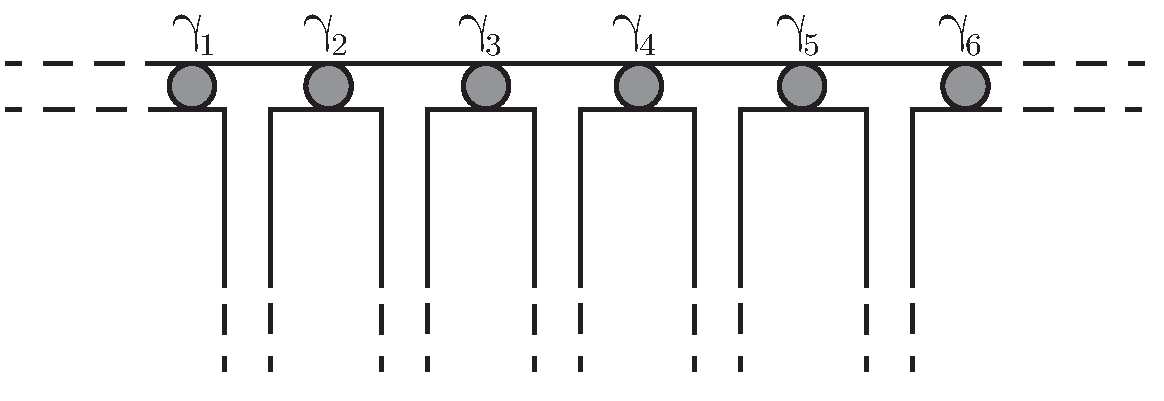
\includegraphics[width=0.95\textwidth]{chapter_introduction/figures/T-junction-network.pdf}
\centering{}
\caption{Majorana T-junction.
The circles represent the Majoranas $\gamma_{1}...\gamma_{6}$.
This network of nanowires allows for the exchange of two Majoranas without having them collide.
This is possible by temporarily bringing a Majorana to one of the vertical wires and then swapping the position of the other Majorana.
\label{fig:Majorana-T-junction}}
\end{center}
\end{figure}
The only thing distinguishing the Majoranas is their position.
That means that after exchanging two Majoranas in space, the system looks identical to the way it looked before the exchange.
We now assume the energy spectrum is gapped for $|E|<\Delta$ with the Majorana ground state at $E=0$.
If this ground state contains several Majoranas, all at zero energy, they form a ``ground state manifold.''

\co{We consider $N$ Majoranas and write down its state of fermionic modes.}
From now on, we only consider the states corresponding to the Majoranas and neglect the states that live in the bulk ($E \geq \Delta$).
As mentioned in Sec.\ref{sec:topology_intro}, a Majorana only has half a degree of freedom, and thus, they can only be assigned quantum states in pairs.
In Fig.~\ref{fig:Majorana-T-junction} we see six Majoranas (3 pairs), but for generality lets consider $N$ pairs.
By pairing two Majoranas (two times half a degree of freedom), we form fermionic modes that give two possible degenerate quantum states, either unoccupied $\ket 0$ or occupied $\ket 1$.
By pairing up neighboring Majoranas $\gamma_{2n-1}$ and $\gamma_{2n}$, we get a creation operator that is its own complex conjugate $c_{n}^{\dagger}=\tfrac{1}{2}(\gamma_{2n-1}+i\gamma_{2n})$, where $c$ is a fermionic creation operator.
Each pair gives two possible quantum states, so $N$ pairs will have $2^{N}$ possible states.
We can represent every state with a ket
\begin{equation}
\left|s_{1},s_{2},\dots,s_{N}\right\rangle,
\end{equation}
where $s_{n}$ is either unoccupied $0$ or occupied $1$.
These states form a complete basis of the Hilbert space.

\co{The parity of the groundstate is an observable.}
We define the fermion parity operator
\begin{equation}
P_{n}\equiv1-2c_{n}^{\dagger}c_{n}=i\gamma_{2n-1}\gamma_{2n},
\end{equation}
that acts on the states and where we recognize the $c_{n}^{\dagger}c_{n}$ term as the number operator.
All basis states in the Hilbert space of the Majoranas are eigenstates of $P_{n}$.
For example, we have
\begin{subequations}
\begin{equation}
P_{1}\left|0,\dots\right\rangle \ =(1-2c_{1}^{\dagger}c_{1})\left|0,\dots\right\rangle =+\left|0,\dots\right\rangle ,
\end{equation}

\begin{equation}
P_{1}\left|1,\dots\right\rangle \ =(1-2c_{1}^{\dagger}c_{1})\left|1,\dots\right\rangle =-\left|1,\dots\right\rangle .
\end{equation}
\end{subequations}
Another important property of Majoranas is that a pair of Majorana operators all anti-commute with each other.
So
\begin{equation}
(\gamma_{1}\gamma_{2})(\gamma_{3}\gamma_{4})=(\gamma_{3}\gamma_{4})(\gamma_{1}\gamma_{2}),
\end{equation}
however, if the pairs share a Majorana, they do not commute anymore, like
\begin{equation}
(\gamma_{1}\gamma_{2})(\gamma_{2}\gamma_{3})=-(\gamma_{2}\gamma_{3})(\gamma_{1}\gamma_{2}).
\end{equation}
Section~\ref{sec:superconductivity} introduced the Hamiltonian Eq.~\eqref{eq:H_BdG_sc}, which does not conserve particle number; however, it conserves the parity.
To calculate the total parity we multiply all parity operators
\begin{equation}
P_{\textrm{tot}}=P_{1}\cdot P_{2}\cdot\,\dots\,\cdot P_{N}=i^{N}\gamma_{1}\gamma_{2}\dots\gamma_{2N},
\end{equation}
where $P_{\textrm{tot}}$ has eigenvalues $\pm1$.
Because the parity is Hermitian, it's observable and equivalently, can be measured experimentally.

\co{We can deduce the braiding operator that exchanges two Majoranas.}
We can now start to think about what happens when we exchange two Majoranas~\cite{Ivanov2001}.
Our ground state manifold $\ket\Psi$ never leaves the ground state if we perform the exchange slowly enough.
The exchange of two Majoranas $\gamma_{n}$ and $\gamma_{m}$ changes the ground state $\left|\Psi\right\rangle \to U\left|\Psi\right\rangle $ where $U$ is a unitary operator.
The exact form of $U$ can be derived without a direct calculation.
We do this by assuming that $U$ only depends on the Majoranas involved in the exchange ( $\gamma_{n}$ and $\gamma_{m}$) and by using that the slow exchange does not change the parity of the system because the system stays gapped at all times.
Since the parity is conserved, we know that $U$ commutes with the total fermion parity $[U,P_{\textrm{tot}}]=0$, and that $U$ can only depend on the product $i\gamma_{n}\gamma_{m}$.
This product is Hermitian, so we can create a unitary operator by taking the exponential of $i$ times this Hermitian operator as
\begin{equation}
U\equiv\exp(\beta\gamma_{n}\gamma_{m})=\cos(\beta)+\gamma_{n}\gamma_{m}\sin(\beta),
\end{equation}
where $\beta$ is a real coefficient.
In the last equality we used $(\gamma_{n}\gamma_{m})^{2}=\gamma_{n}\gamma_{m}\gamma_{n}\gamma_{m}=-\gamma_{n}\underset{=1}{\underbrace{\gamma_{m}\gamma_{m}}}\gamma_{n}=-1$
in the Taylor expansion.
We now move to the Heisenberg picture where we look at the evolution of the Majorana operators in time
\begin{subequations}
\begin{equation}
\gamma_{n}\to U\gamma_{n}U^{\dagger}=\left(\cos\beta+\gamma_{n}\gamma_{m}\sin\beta\right)\gamma_{n}\left(\cos\beta+\gamma_{m}^{\dagger}\gamma_{n}^{\dagger}\sin\beta\right),
\end{equation}

\begin{equation}
=\gamma_{n}\cos^{2}\beta+\left(\gamma_{n}\gamma_{m}^{\dagger}\gamma_{n}^{\dagger}+\gamma_{n}\gamma_{m}\gamma_{n}\right)\sin\beta\cos\beta+\gamma_{n}\gamma_{m}\gamma_{n}\gamma_{m}^{\dagger}\gamma_{n}^{\dagger}\sin^{2}\beta,
\end{equation}

\begin{equation}
=\gamma_{n}\cos^{2}\beta-\gamma_{n}^{\dagger}\sin^{2}\beta-2\gamma_{m}\sin\beta\cos\beta,
\end{equation}

\begin{equation}
=\gamma_{n}\cos2\beta-\gamma_{m}\sin2\beta.
\end{equation}
\end{subequations}
In a similar way, we get
\begin{equation}
\gamma_{m}\to U\gamma_{m}U^{\dagger}=\gamma_{m}\cos2\beta+\gamma_{n}\sin2\beta.
\end{equation}
After the exchange happened we know that $\gamma_{m}\to\gamma_{n}$ and $\gamma_{n}\to\gamma_{m}$, which means that $\beta=\pm\pi/4$.
The two opposite signs distinguish the clockwise and the counterclockwise exchange of the Majoranas.
We now found an operator that exchanges two Majoranas
\begin{equation}
U=\exp\left(\pm\frac{\pi}{4}\gamma_{n}\gamma_{m}\right)=\tfrac{1}{\sqrt{2}}\left(1\pm\gamma_{n}\gamma_{m}\right).\label{eq:U_nm}
\end{equation}

\co{As an example, we apply this operator to the simplest non-trivial case of having just four Majoranas.}
As an example, we consider just four Majoranas $\gamma_{1}$, $\gamma_{2}$, $\gamma_{3}$, and $\gamma_{4}$ and exchange their positions.
The four basis states in the ground state manifold are
\begin{equation}
\left|00\right\rangle ,\left|01\right\rangle ,\left|10\right\rangle ,\left|11\right\rangle ,\label{eq:basis}
\end{equation}
where the first number is the occupation number of the fermionic mode $c_{1}^{\dagger}=\tfrac{1}{2}(\gamma_{1}+i\gamma_{2})$ and the second number the occupation number of $c_{2}^{\dagger}=\tfrac{1}{2}(\gamma_{3}+i\gamma_{4})$.
For instance, if we start from the state $\left|00\right\rangle $ and we exchange $\gamma_{2}$ and $\gamma_{3}$ by applying $U_{23}=\tfrac{1}{\sqrt{2}}\left(1\pm\gamma_{2}\gamma_{3}\right)$, we obtain
\begin{equation}
\left|00\right\rangle \to U_{23}\left|00\right\rangle =\tfrac{1}{\sqrt{2}}\left(\left|00\right\rangle +i\left|11\right\rangle \right).
\end{equation}  % XXX: check how this exactly works, and maybe add more details?
Here we see a superposition of states, which is not like bosons or fermions, where the exchange only changes the sign.
Because of this property, Majoranas are non-Abelian anyons.
As noted before, exchanging two non-Abelian anyons is called braiding.
Using these braiding operations, it is possible to create a qubit that can perform a certain set (but not all) of rotations on the single-qubit Bloch sphere.
This means that some of the qubit operations are topologically protected.
This reduces the amount of error-correction needed in comparison with a non-topological qubit, and in turn, means that fewer physical qubits are required.


%%%%%%%%%%%%%%%%%%%%%%%%%%%%%%%%%%%%%%%%%%%%%%%%%%%%%%%%%%%%%%%%%%%%%%%%%%%%%%%%%%%%%%%
%%%%%%%%%%%%%%%%%%%%%%%%%%% MAJORANAS IN A MINIMAL NANOWIRE %%%%%%%%%%%%%%%%%%%%%%%%%%%
%%%%%%%%%%%%%%%%%%%%%%%%%%%%%%%%%%%%%%%%%%%%%%%%%%%%%%%%%%%%%%%%%%%%%%%%%%%%%%%%%%%%%%%


\section{Majoranas in a minimal hybrid nanowire}\label{sec:minimal_majoranas}
\co{Superconductivity, spin-orbit coupling, a Zeeman field, and tuned µ leads to the appearance of Majoranas near the edges of the wire.}
The combined effect of superconductivity, spin-orbit coupling, and a Zeeman field can lead to the appearance of Majoranas near the edges of the wire~\cite{Lutchyn2010,Oreg2010}.
To understand how this happens, we study the effects of the various terms in the Hamiltonian.
As discussed in Sec.~\ref{sec:topology_intro}, the appearance of Majoranas is a topological effect and is accompanied by the change of the topological invariant $Q$ of symmetry class $\mathcal{D}$.
This invariant can only assume $Q=+1$ (no Majoranas) and $Q=-1$ (Majoranas present) and changes when the band gap closes and reopens.

\begin{figure}
\begin{center}
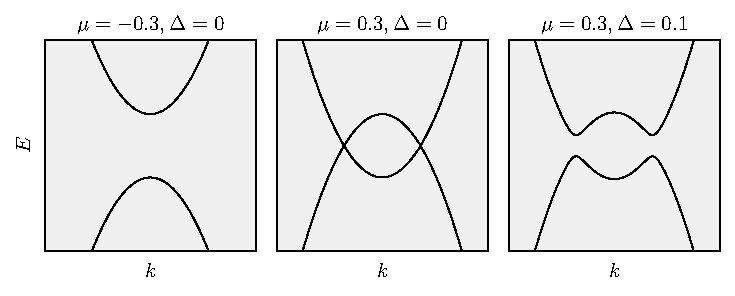
\includegraphics[width=0.95\textwidth]{chapter_introduction/figures/triv_topo_bandstructure.pdf}
\caption{Band structures of Hamiltonians with chemical potential $\mu=-0.3$ and superconducting gap $\Delta=0$ (left); $\mu=0.3$ and $\Delta=0$ (middle); and $\mu=0.3$ and $\Delta=0.1$ (right).
\label{fig:triv_topo_bandstructure}}
\end{center}
\end{figure}

\subsection{The Hamiltonian: term by term}\label{sec:hamiltonian_term_by_term}
\co{We show what the effect of these individual terms is on the band structure.}
The complete model Hamiltonian is rather complicated; therefore, we start with a one-dimensional single band Hamiltonian and study its band structure while adding the terms needed to make a topological band structure and ``engineer'' our way towards Majoranas.
The Hamiltonian in its simplest form is quadratic in momentum and has an off-set in chemical potential $\mu$
\begin{equation}
H=\left(\frac{\bm{p}^{2}}{2m}-\mu\right)\tau_{z},\label{eq:simple_ham}
\end{equation}
where $\tau_{z}$ is a Pauli matrix that acts on the electron-hole substructure.
The band structure for this Hamiltonian with $\mu=-0.3$ is shown in Fig.~\ref{fig:triv_topo_bandstructure} (left).
We assume that this band structure is topologically trivial and has $Q=+1$.
Because this Hamiltonian acts trivially in spin-space, the bands in Fig.~\ref{fig:triv_topo_bandstructure} (left) are doubly degenerate.
Finally, the electrons are at positive energy $E$ and the holes on $-E$.

\co{We require a band gap, so we add superconductivity, resulting in a BdG Hamiltonian with a gapped spectrum.}
Next, we raise $\mu$, which shifts the bands [see Fig.~\ref{fig:triv_topo_bandstructure} (middle)].
In Sec.~\ref{sec:topology_intro}, we explained that the topological invariant is only defined for a system with an energy gap.
This band structure has no band gap, and therefore cannot be topological.
Further, in Sec.~\ref{sec:superconductivity} we observed that a BdG Hamiltonian has a gapped spectrum [Eq.~\eqref{eq:SC_spectrum}], so we add $\Delta\tau_{x}$, which results in
\begin{equation}
H_{\textrm{BdG}}=\left(\frac{\bm{p}^{2}}{2m}-\mu\right)\tau_{z}+\Delta\tau_{x},
\end{equation}
and opens a gap because $\tau_{x}$ mixes the electron and holes [see Fig.~\ref{fig:triv_topo_bandstructure} (right)].

\co{We break the spin degeneracy using a magnetic field.}
We are left with a gapped spectrum; however, we closed the band gap twice because of the doubly degenerate spin bands both crossing zero energy simultaneously.
The spin degeneracy (called a Kramers degeneracy\footnote{A Kramers degeneracy would result in two Majoranas per edge (just a fermion).}) is a result of a time-reversal symmetry and needs to be broken to create isolated Majoranas.
To couple to spin we introduce the Zeeman field $E_\textrm{Z}\sigma_{x}=\frac{1}{2}g\mu_{\textrm{B}}B\sigma_{x}$ in the Hamiltonian
\begin{equation}
H_{\textrm{BdG}}=\left(\frac{\bm{p}^{2}}{2m}-\mu\right)\tau_{z}+\Delta\tau_{x}+\frac{1}{2}g\mu_{\textrm{B}}B\sigma_{x},\label{eq:zeeman}
\end{equation}
where $g$ is the Landé factor, $\mu_{\textrm{B}}$ the Bohr magneton, and $B$ magnetic field along $x$, parallel to the wire direction.
In Fig.~\ref{fig:zeeman} we plot the effect of a magnetic field on the band structure and observe that a magnetic field breaks the Kramers degeneracy.
\begin{figure}
\begin{center}
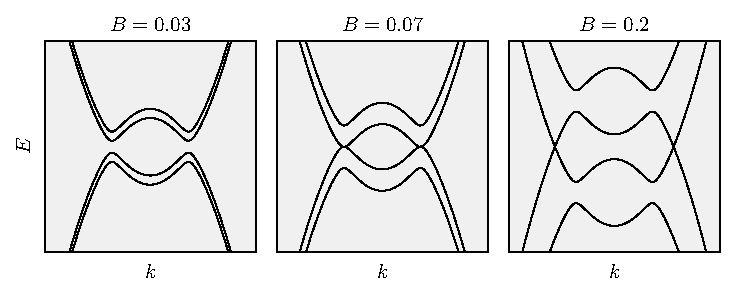
\includegraphics[width=0.95\textwidth]{chapter_introduction/figures/zeeman.pdf}
\caption{Band structures of Eq.~\eqref{eq:zeeman} for different values of magnetic field and $\Delta=0.1$, $\mu=0.3$.
\label{fig:zeeman}}
\end{center}
\end{figure}
The bands moving towards each other have opposite spin (orthogonal states), and as we see in Fig.~\ref{fig:zeeman} (middle and left), these spins do not couple.
The problem is that Zeeman conserves spin in $x$-direction, and therefore spin is still a good quantum number.
We know that Majoranas must be spinless because they are their own complex conjugate.

\co{To break spin-rotation symmetry, we introduce the spin-orbit coupling, which by itself is not enough to create Majoranas.}
The solution to this last problem is spin-orbit coupling, which in its simplest form is Rashba: $H_{\textrm{Rashba}}=-\alpha p_{x}\sigma_{y}\tau_{z}$.
The Hamiltonian is now complete and equals
\begin{equation}
H_{\textrm{BdG}}=\left(\frac{\bm{p}^{2}}{2m}-\mu\right)\tau_{z}+\Delta\tau_{x}+\frac{1}{2}g\mu_{\textrm{B}}B\sigma_{x}-\alpha p_{x}\sigma_{y}\tau_{z}.\label{eq:rashba}
\end{equation}
Spin-orbit by itself---eventhough it couples spin---is insufficient to break the Kramers degeneracy.
In Fig.~\ref{fig:SO_no_zeeman}, we see that raising $\alpha$ moves the different spin bands away in either $+k$ or $-k$ direction.
However, a degeneracy remains at $k=0$, revealing why a magnetic field is needed.
\begin{figure}
\begin{center}
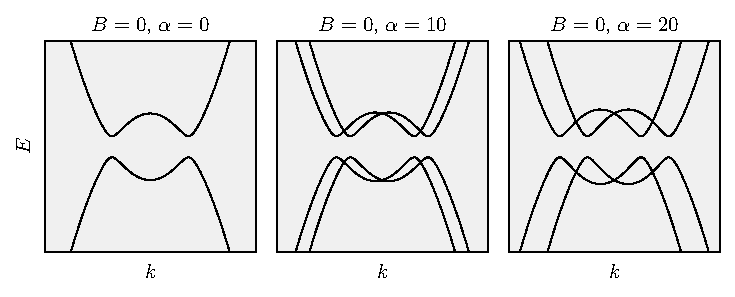
\includegraphics[width=0.95\textwidth]{chapter_introduction/figures/SO_no_zeeman.pdf}
\caption{Band structures of Eq.~\eqref{eq:rashba} for different values of spin-orbit coupling $\alpha$ and $B=0$, $\Delta=0.1$, $\mu=0.3$.
\label{fig:SO_no_zeeman}}
\end{center}
\end{figure}
Including a magnetic field opens the gap at $k=0$ (see Fig.~\ref{fig:SO_and_zeeman}) making the system topologically nontrivial.
If the system is of a finite length, it will host Majoranas on its edges at $E=0$.
\begin{figure}
\begin{center}
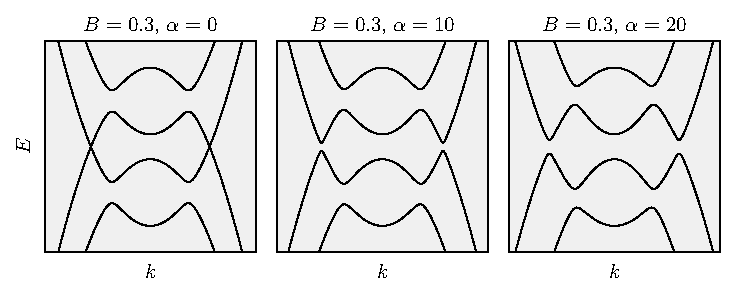
\includegraphics[width=0.95\textwidth]{chapter_introduction/figures/SO_and_zeeman.pdf}
\caption{Band structures of Eq.~\eqref{eq:rashba} for different values of spin-orbit coupling $\alpha$ and $B=0.3$, $\Delta=0.1$, $\mu=0.3$.
\label{fig:SO_and_zeeman}}
\end{center}
\end{figure}

\subsection{Wavefunction}
\co{Using the right parameters, we can plot the Majorana wavefunction.}
We now have all the terms in the Hamiltonian to create a topological band structure, which we calculate for an infinite system (i.e., system with a translational symmetry).
To observe Majoranas, we need to diagonalize the Hamiltonian of a finite system with the same parameters that resulted in the topological band structure and plot the wavefunction with the lowest energy: the Majorana wavefunction.
In Fig.~\ref{fig:wavefunction_1d} (left), we plot the probability density of the Majorana wavefunction and observe that it is indeed localized near edges of the nanowire.
This wavefunction decays exponentially from both sides with a decay length $\xi_\textrm{M}$.

\begin{figure}
\begin{center}
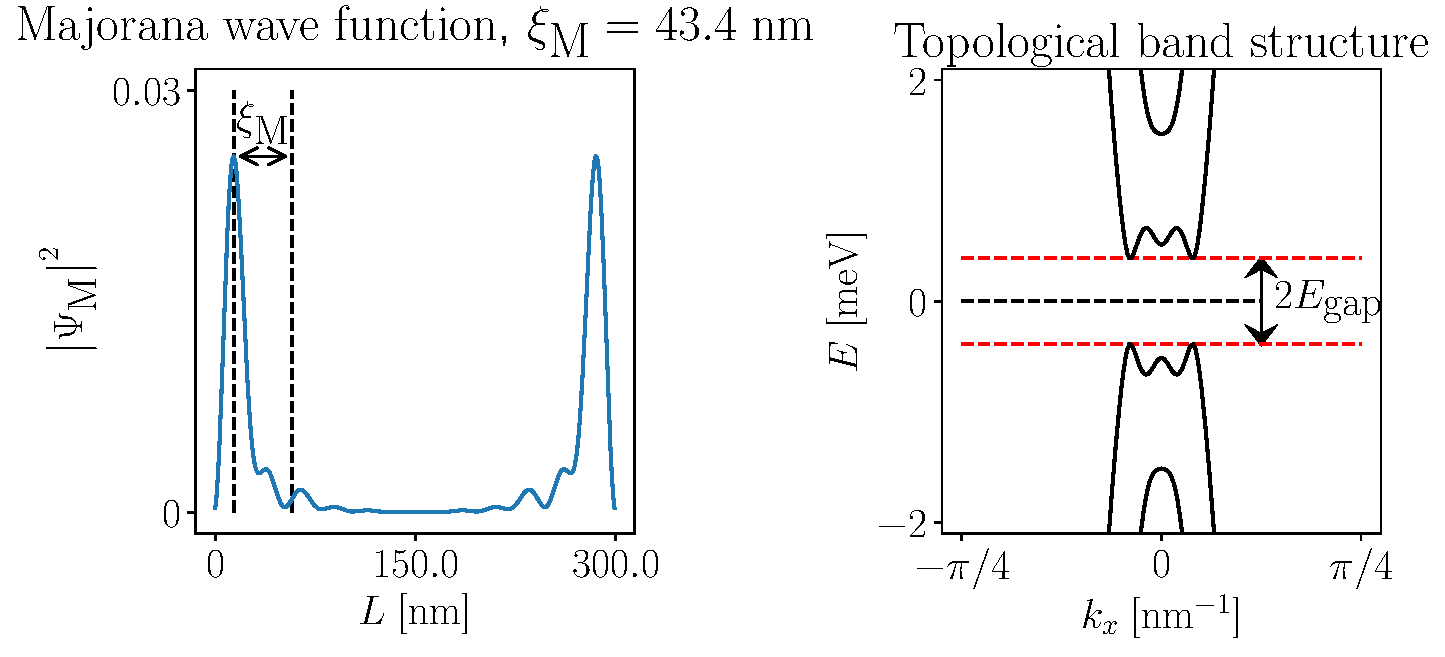
\includegraphics[width=0.95\textwidth]{chapter_introduction/figures/wf_and_band_structure.pdf}
\caption{Probability density and band structure of a 1D system.
The probability density of the lowest energy wavefunction (Majorana wavefunction) of a \SI{0.3}{\micro\metre} long nanowire (left) and a topological band structure (right) with the same parameter values, but for an infinite system.
The Majorana length $\xi$---the decay length of the wavefunction---in the left plot is $\xi_\textrm{M}=\SI{43.4}{nm}$.
\label{fig:wavefunction_1d}}
\end{center}
\end{figure}

\subsection{Phase diagram}\label{sec:phase_diagram_1D_intro}
\co{With a phase diagram, we show for which tunable parameters the system is topological.}
The Hamiltonian [Eq.~\eqref{eq:rashba}] contains a few fundamental constants and constants that are material dependent; however, the chemical potential $\mu$ and magnetic field $B$ can be adjusted in an experiment.
A good question is, for which values of $B$ and $\mu$ the system is topological.
Due to its compactness, this model can be solved analytically, and it predicts that Majorana bound states appear when $E_\textrm{Z}^{2}>\mu^{2}+\Delta^{2}$, when the Zeeman energy becomes larger than the harmonic mean of the superconducting gap and the chemical potential.
In Fig.~\ref{fig:phase_diagram_1D} we plot a phase diagram, which indicates for which value of $\left(B,\; \mu\right)$ the system is topological.
In the next section, we will extend this model to three dimensions and study how it modifies the phase diagram.

\begin{figure}
\begin{center}
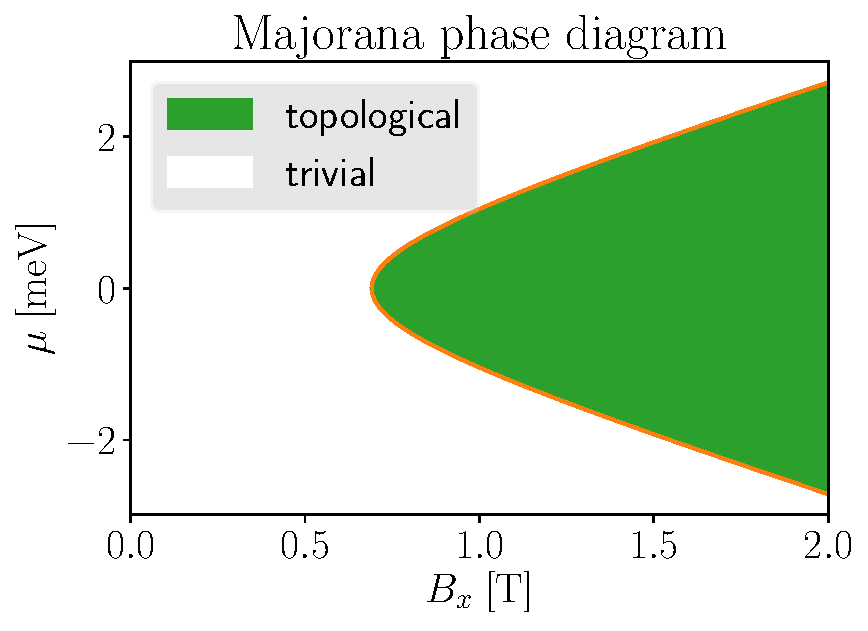
\includegraphics[width=0.7\textwidth]{chapter_introduction/figures/phase_diagram_1D.pdf}
\caption{A phase diagram of a one-dimensional Majorana nanowire device as a function of magnetic field $B$ and chemical potential $\mu$.
The color indicates whether the system is in the topological or trivial phase.
This system becomes topological whenever $E_\textrm{Z}^{2}>\mu^{2}+\Delta^{2}$.
\label{fig:phase_diagram_1D}}
\end{center}
\end{figure}


%%%%%%%%%%%%%%%%%%%%%%%%%%%%%%%%%%%%%%%%%%%%%%%%%%%%%%%%%%%%%%%%%%%%%%%%%%%%%%%%%%%%%%%
%%%%%%%%%%%%%%%%%%%%%%%%% MAJORANAS IN A REALISTIC 3D NANOWIRE %%%%%%%%%%%%%%%%%%%%%%%%
%%%%%%%%%%%%%%%%%%%%%%%%%%%%%%%%%%%%%%%%%%%%%%%%%%%%%%%%%%%%%%%%%%%%%%%%%%%%%%%%%%%%%%%


\section{Majoranas in a more realistic 3D hybrid nanowire}\label{sec:realistic_nanowire}
\co{The simple model is great, but experiments does not agree, so we need to include more physical effects.}
The simple one-dimensional model we introduced in the previous section is useful because it can be solved analytically and therefore, it gives us many insights.
However, because of its simplicity, it also ignores multiple relevant physical effects.
For example, the model assumes a one-dimensional nanowire even though we live in a three-dimensional world, and so does the nanowire device when an experimentalist creates it.
Besides the additional orbitals that are present in a three-dimensional system, the magnetic flux penetrating the nanowire cross-section modifies the Hamiltonian and changes the complex phases of the moving quasiparticles.
Further, the simple model assumes a tunable but constant chemical potential $\mu$ inside the nanowire.
In an experiment, the nanowire is close to a metal gate at a certain voltage; its electric field changes the potential inside the nanowire non-homogeneously.
In addition to these theoretical considerations, the experimental measurement results do not correspond to the predictions that the simple model makes.
For example, for measuring the conductance from a nanowire hosting Majoranas to a normal lead, the model predicts a quantized conductance of $2 e^2/h$ at a bias voltage of $V_\textrm{B}=0$, the so-called zero-bias peak.
Nearly all experiments \footnote{not arXiv:1710.10701} that measure this fail to reproduce this zero-bias peak where the conductance is quantized.
Another effect that is not captured by the simple model is the superconducting density of states (DOS), which in theory predicts a vanishing DOS inside the gap ($|E|<\Delta$) but the experiment a non-zero DOS persists, this phenomenon is also called ``soft gap.''
Because of these limitations, we will improve the simple model by adding relevant physical effects.

\subsection{Multiple bands}
\co{In 3D more orbitals are present, breaking the simple E_z²>µ²+Δ² requirement for Majoranas.}
In 3D, the model Hamiltonian [Eq.~\eqref{eq:rashba}] is modified to
\begin{equation}
H_{\textrm{BdG}}=\left(\frac{\bm{p}^{2}}{2m}-\mu\right)\tau_{z}+\Delta\tau_{x}+\frac{1}{2}g\mu_{\textrm{B}}B\sigma_{x}+\alpha\left(p_{y}\sigma_{x}-p_{x}\sigma_{y}\right)\tau_{z},\label{eq:3D_Ham}
\end{equation}
such that it includes the transverse part of the Rashba spin-orbit.
The two additional dimensions result in more orbitals and equivalently more bands; therefore, the condition $E_\textrm{Z}^{2}>\mu^{2}+\Delta^{2}$ for a topological nanowire is no longer valid.
Because there are more bands, multiple Majoranas can be created on both edges of the nanowire as $\mu$ increases.
However, these additional Majoranas are not topologically protected (without an additional symmetry), and a small perturbation can pair-wise annihilate all but $N \mod 2$ of them.
The position of the phase boundaries now also depends on the cross-section's geometry.
For example, Fig.~\ref{fig:topo_bands} shows a phase diagram (and band structures at different combinations of $B$ and $\mu$) of a nanowire with a cylindrical cross-section.
\begin{figure}
\begin{center}
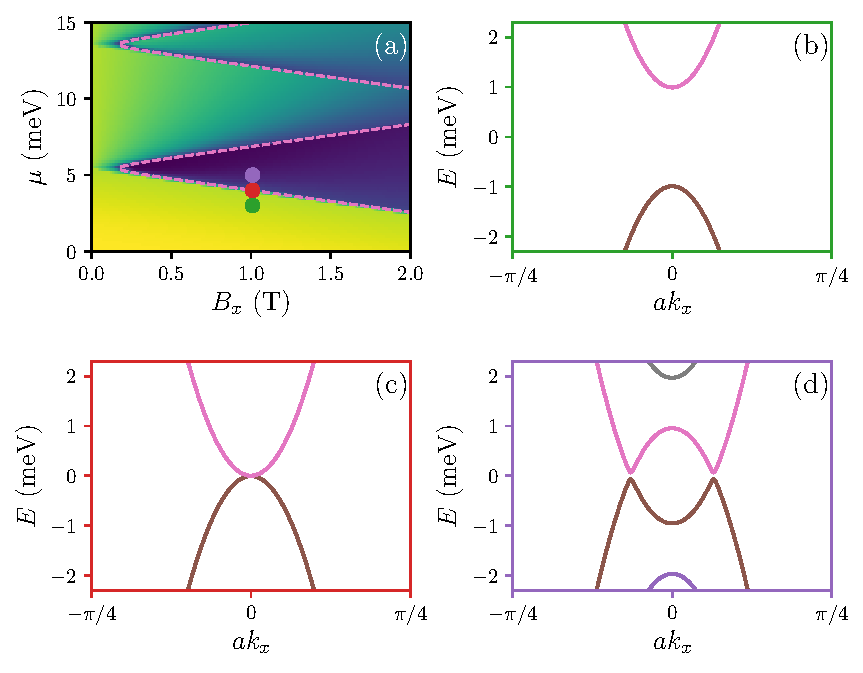
\includegraphics[width=0.8\textwidth]{chapter_introduction/figures/phase_diagram_with_bands.pdf}
\caption{Topological phase diagram (a) of a 3D system where the dot indicate the parameter values of $B,\; \mu$ at which the surrounding band structures (b-d) are plotted.
The color in the phase diagram (a) shows the size of the topological gap $E_\textrm{gap} \equiv \min_k E(k)$ and the dashed lines are the topological phase boundaries.
The band structure (b) is trivial but near a phase transition, (c) is at the phase transition, and (d) is inside of the topological regime.
\label{fig:topo_bands}}
\end{center}
\end{figure}

\subsection{The orbital effect of the magnetic field}\label{sec:orbital_effect_of_magnetic_field}
\co{Whenever a magnetic flux can penatrate the nanowire, the canonical momentum operator is modified to include the vector potential.}
Whenever a magnetic flux can penatrate a surface of the nanowire, the canonical momentum operator in Eq.~\eqref{eq:3D_Ham} is modified to include the vector potential
\begin{equation}
\bm{p} \rightarrow -i \hbar \nabla - q \bm{A} \tau_z,\label{eq:continuum_kinetic_with_orbital}
\end{equation}
where $q$ is the elementary charge, which is different for electrons and holes.
In the weak coupling regime---with a non transparent semiconductor/superconductor interface---and a wire that is symmetric with respect to the wire axis, the vector potential is $\mathbf{A}={\left[ B_y (z - z_0) - B_z (y - y_0), 0, B_x (y - y_0)\right]}^{T}$, which is chosen such that it does not depend on $x$.
Here, we set the offsets $y_0$ and $z_0$ such that the average vector potential vanishes in the superconductor.
Physically, this choice corresponds to a limit where the total supercurrent $J_s$ is zero, appropriate for existing devices that use NbTiN as a superconducting shell.
In this case, the superconductor can be considered as a perturbation that only provides the electron-hole coupling in the normal regime.
However, devices that have a thin Al shell are in the strong coupling regime.
Because of the high density inside the superconductor (compared to the semiconductor), the wire can no longer be considered as symmetric with respect to the wire axis.
To get correct physical observables from both the vector potential and the superconducting phase difference $\theta$~\cite{Wojcik2018}, we have to ensure that the total supercurrent cancels out,
\begin{equation}
\bm{J}_s = \frac{2e n_s}{m}\left(2e \bm{A} - \hbar \nabla \Phi \right)=0,
\end{equation}
where $n_s$ is the density in the superconductor.
At zero temperature, this can be archived by minimizing the kinetic energy, which is proportional to $E_s \propto \int d \bm{x} J_s^2(\bm{x})$ ~\cite{Winkler2019}.
This minimization results in the correct vector potential and the superconducting phase.
The inclusion of the orbital effect modifies the phase diagram, which is discussed in Ch.~\ref{ch:orbitalfield} in the weakly coupled superconductor limit, while Ch.~\ref{ch:shortjunction} discusses the strongly coupled superconductor limit.

\subsection{Disorder}
\co{A real system's material is not perfectly smooth and has impurities, and we can model this disorder by random onsite energy.}
Perfectly ordered crystalline solids are characterized by a faultlessly regular arrangement of their atoms in a crystal lattice, yet, these do not occur in nature~\cite{Nolting1970}.
Real solid-state systems are not perfectly smooth and have impurities: they are disordered.
Disorder is always present and it has a strong impact on the physical properties of proximitized nanowires.
Research has shown that both disorder in the semiconductor and at the semiconductor-superconductor interface is detrimental to the creation of Majoranas in proximitized nanowires~\cite{Lobos2012,Lutchyn2012,Sau2012a,Sau2013,Hui2015,Cole2016,Liu2018}.
However, semiconductor nanowire with epitaxially grown aluminium~\cite{Lutchyn2018,Krogstrup2015} minimize the disorder effects and have high-quality semiconductors and semiconductor-superconductor interfaces; however, its outer surface is oxidized and therefore strongly disordered.
Scattering of the disordered superconducting boundary randomizes the quasiparticle's motion inside the superconductor.
Fortunately, because of the large difference in the effective masses and Fermi energies between the semiconductor and the superconductor, as argued by the authors of~\cite{Sticlet2017,Lutchyn2012,Liu2018}, disorder in the superconductor is not detrimental to the manipulation and observation of Majoranas, however, a more systematic numerical study is required.
This problem is complex to study numerically because of the aforementioned high density differences, which means that the discretization in the superconductor has to be smaller than the Fermi wavelength of Al, $\approx \SI{0.1}{\AA}$.
A full-scale three-dimensional simulation is therefore beyond what is currently feasible.
Nevertheless,~\cite{Antipov2018} simulates a slice of the proximitized nanowire, and finds that disorder strongly affects important quantities such as the induced gap $\Delta_\textrm{ind}$, the critical field $B_\textrm{c}$, and their dependence on the external gate voltage.

\subsection{Electrostatics}
\co{Majorana device proposals rely on a fine control of the electrostatics and understanding what happens is complicated.}
The model Hamiltonian Eq.~\eqref{eq:3D_Ham} has a constant chemical potential $\mu$ in the nanowire.
Experimentally, $\mu$ is set by the external metal gates that, when applying a voltage, will change the electrostatic environment inside the device.
Therefore, we replace the static chemical potential by a spatially dependent electrostatic potential $\mu \rightarrow -V(x, y, z)$ in the Hamiltonian.
Recent proposals of scalable designs for topological quantum computing with Majoranas rely on a precise electrostatic control.
A good understanding of how the metal gates influence the electrostatic potential is therefore required to interpret both existing Majorana experiments and future improved Majorana devices.
One of the challenges is that the metal gates have band offsets in the 1-eV range, while a typical semiconductor's Fermi energy lies in the 1-meV range, three orders of magnitude difference~\cite{Armagnat2019}.
Additionally, as mentioned in Sec.~\ref{sec:braiding}, the BCS mean-field approximation breaks charge conservation.
We can formulate the quantum-electrostatic problem as a solution of three equations solved self-consistently.
We have the Schrödinger equation
\begin{equation}
H_\textrm{BdG} \psi = E \psi,\label{eq:schrodinger}
\end{equation}
the Poisson equation
\begin{equation}
\nabla^2 \varphi = -\frac{\rho }{\varepsilon},\label{eq:poisson}
\end{equation}
where $\varepsilon$ is the permittivity, and the density of states is
\begin{equation}
\rho = e \int dE \rho_i(E) f(E),\label{eq:DOS}
\end{equation}
where $f(E)$ is the Fermi distribution and $\rho_i(E) \equiv \frac{1}{2\pi} \sum_\alpha {\left| \psi_{\alpha E}(i) \right|}^2$ the local density of states.
Using these equations, one can iterate the following steps until convergence has been reached:
\begin{enumerate}
\item given the electronic density, solving the Poisson equation [Eq.~\eqref{eq:poisson}] results in the electrostatic potential,
\item given the electrostatic potential $V(x, y, z)$, solving the Schrödinger equation [Eq.~\eqref{eq:schrodinger}] results in the energy spectrum $E$ and wave functions $\psi$,
\item finally, using that the bands fill according to the Fermi distribution $f(E)$, we get the electronic density [Eq.~\eqref{eq:DOS}].
\end{enumerate}
Several works have solved this problem, however, always using certain approximations.
For example,~\cite{Vuik2016} does this in the long junction or weakly coupled regime for a translationally invariant slice of the system.
Other works try to solve this problem for the short junction or strongly coupled regime, also only simulating the cross-section of the nanowire~\cite{Antipov2018}, and/or by employing the Thomas-Fermi approximation~\cite{Mikkelsen2018,Winkler2019} (with which one can replace step 2.~and 3.~by using a scalar equation that returns the density $\rho$,) or by using other approximations~\cite{Escribano2017,Dominguez2017,Woods2018}.
These works find that applying a voltage on external metal gates renormalizes several important physical parameters, such as the induced superconducting gap $\Delta_\textrm{ind}$ and the critical magnetic field $B_\textrm{c}$, and in turn, this means that the phase diagram changes.
Due to the extreme computational complexity, no one has solved the full three-dimensional Schrödinger-Poisson problem, while treating the superconductor and semiconductor on equal footing.

\subsection{Superconducting order parameter}
\co{The superconducting order parameter is assumed to be constant, however, it is not clear if this assumption is valid.}
In most studies~\cite{Antipov2018,Winkler2019,Vuik2016,Nijholt2016,Winkler2017}, the superconducting order parameter $\Delta$ is assumed to be constant inside the superconductor, even though an applied magnetic field might cause a spatial variation in both $\Delta$'s phase $\phi$ and amplitude.
One possible reason for this is the Meissner effect, where the superconductor (below its critical temperature $T_\textrm{c}$) develops a supercurrent and expels the magnetic field.
When the applied magnetic field $B$ is large, vortices appear, which in the center have $\Delta=0$ and allow magnetic flux to penetrate the superconductor.
In turn, this suppresses the induced superconducting gap $\Delta_\textrm{ind}$ locally, which creates unwanted subgap states in the superconductor.
Ginzburg-Landau theory captures vortex formation.
Section~\ref{sec:spin_orbit_supplemental_theory} investigates this for a NbTiN superconductor where the superconducting penetration depth $\lambda$ is approximately three times smaller than the thickness of the superconductor and find that the vortices that appear do not have a substantial effect on the size of the induced gap.
However, the epitaxially grown aluminum is much thinner (typically $\approx \SI{10}{\nm}$).
In this case, $\lambda$ is much larger, resulting in a uniform magnetic field inside the superconductor.
Here, the orbital effect of the magnetic field needs to be adequately treated, which is done by the authors of~\cite{Winkler2019,Wojcik2018}, as discussed earlier.
In principle, the amplitude $\left| \Delta \right|$ is also spatially dependent, and can be solved self-consistently as it often done in ferromagnetic chains on superconductors~\cite{Awoga2017,Sacramento2007}.
However, in the case of hybrid semiconductor-superconductor systems, it is shown that this effect is less significant~\cite{Awoga2019}.

\subsection{Spin-orbit coupling}
\co{Spin-orbit coupling is a crucial to create Majoranas, we can model it better by using with k.p methods.}
Finally, the presence of strong spin-orbit coupling is crucial to create Majoranas.
The Rashba spin-orbit term $\alpha\left(p_{y}\sigma_{x}-p_{x}\sigma_{y}\right)$ in Eq.~\eqref{eq:3D_Ham} can be derived in the framework of the k$\cdot$p perturbation theory.
Intuitively, it can be understood as an effective magnetic field that is the result of an inversion symmetry breaking electric field along the $z$ axis $H_E=-E_0 z$.
An electron that moves through this electric field with velocity $v$, experiences an effective magnetic field $\bm{B} =-(\bm{v} \times \bm{E} )/c^{2}$ due to relativistic corrections.
This effective magnetic field couples to the spin as $H_\textrm{SO} = \frac{1}{2} g \mu_\textrm{B} \bm{B} \cdot \bm{\sigma} = -\frac{g \mu_\textrm{B}}{2c^2} (\bm{v} \times \bm{E}) \cdot \bm{\sigma}$.
Combining the constants into $\alpha = g \mu_\textrm{B} E_0 \hbar / 2 m c^2$ results in $H_\textrm{SO}$ that appears in Eq.~\eqref{eq:3D_Ham}.
Therefore, this term assumes a homogeneous electric field, which is the case for a wire with a constant chemical potential $\mu$.
However, as discussed earlier, this is not the case.
The k$\cdot$p perturbation theory that includes multiple conduction and valance bands models the spin-orbit coupling more accurately.
Here, the spin-orbit strength depends on the electric field resulting from the voltage that is applied to the external metal gates.
In addition, k$\cdot$p theory also provides a better model for the effective mass in a semiconductor.
However, describing k$\cdot$p theory is beyond the scope of this thesis.
Finally, as Majorana device simulations become capable of correctly including the spatially varying electric field into their models (as discussed earlier), it enables researchers to understand how this affects the spin-orbit coupling by using the k$\cdot$p theory.


%%%%%%%%%%%%%%%%%%%%%%%%%%%%%%%%%%%%%%%%%%%%%%%%%%%%%%%%%%%%%%%%%%%%%%%%%%%%%%%%%%%%%%%
%%%%%%%%%%%%%%%%%%%%%%%%%%%%%%%%%% NUMERICAL METHODS %%%%%%%%%%%%%%%%%%%%%%%%%%%%%%%%%%
%%%%%%%%%%%%%%%%%%%%%%%%%%%%%%%%%%%%%%%%%%%%%%%%%%%%%%%%%%%%%%%%%%%%%%%%%%%%%%%%%%%%%%%


\section{Numerical methods}\label{sec:numerical_methods}
\co{Finite difference approximation solves the problem when analytical methods fail.}
Section~\ref{sec:realistic_nanowire} shows that realistically modeling Majorana devices is complex and that it is impossible to solve these problems analytically without making simplifications that still capture all of the relevant physics.
Therefore, to study Majorana devices, we must use numerical methods.
Using the finite difference approximation, we can convert the linear ordinary differential equation, the continuous BdG Hamiltonian Eq.~\eqref{eq:3D_Ham}, into a system of equations described by a (potentially very large) sparse matrix.
With readily available standard sparse linear algebra techniques, such as the shift-invert diagonalization method, we can efficiently find low energy wavefunctions of our system.

\subsection{Band structure}\label{sec:band_structure_numerics}
\co{Translationally invariant systems are described with a band structure.}
In principle, to correctly predict device properties, one needs to simulate a large nanowire that includes the edges of the wire.
However, because topology is robust and insensitive to details, we can simulate just the band structure in the bulk of the wire.
From this, we understand whether the system is topological or topologically trivial.
To calculate a band structure $E(k)$, we use Bloch's theorem, which states that the wave function in a crystal changes under translation only by a phase factor
\begin{equation}
\psi(\bm{r}+a) = e^{i a k}\psi(\bm{r}),
\end{equation}
where $k$ is the wave vector of the wave function and $a$ the size of the unit-cell.
This implies that we only need to simulate a translationally invariant unit-cell to get $E(k)$.
The Hamiltonian equals  % XXX: the rest of the section isn't as smooth...
\begin{equation}
H\left(k\right) = h + t\exp(ik) + t^{\dagger}\exp(-ik),
\end{equation}
where $h$ is the Hamiltonian of the cross section of the tight-binding system and $t$ is the hopping matrix between the neighboring cross sections.
Next section explains how to get the tight-binding model.
Diagonalizing this Hamiltonian at $k$ results in the spectrum $E(k)$.
Finally, due to the discretization, the Brillouin zone is periodic.
However, one should be careful to not simulate effects from its corners because the band structure only correctly represents the continuum model near the band bottom.

\subsection{Discretization of the Hamiltonian}
\co{Discretization of the continuous BdG Hamiltonian on to a lattice}
To turn Eq.~\eqref{eq:3D_Ham} into a discretized tight-binding model, we replace $\bm{p} \rightarrow -i\hbar \nabla$, where $\nabla \equiv \left( \frac{\partial}{\partial_x}, \frac{\partial}{\partial_y}, \frac{\partial}{\partial_z} \right) \equiv \left( \partial_x, \partial_y, \partial_z \right)$, to get
\begin{equation}
H_{\textrm{BdG}}=\left(\frac{-\hbar^{2}\nabla^{2}}{2m}-\mu\right)\tau_{z}+\Delta\tau_{x}+\frac{1}{2}g\mu_{\textrm{B}}B\sigma_{x}+i\hbar\alpha\left(\partial_{x}\sigma_{y}-\partial_{y}\sigma_{x}\right)\tau_{z}.\label{eq:3D_Ham_again}
\end{equation}
We discretize the differential operators in $H_{\textrm{BdG}}$ on sites of a square lattice with lattice constant $a$.
Every site is indexed by integer lattice coordinates $(i,j,k)$, which have real-space coordinates $(x,y,z)=(ai,aj,ak)=\bm{r}$.
It is convinient to introduce creation $c^\dagger_{\bm{r}}$ and annihilation $c_{\bm{r}}$ operators that act on the sites, where
\begin{equation}
c_{\bm{r}} \equiv c_{ai, aj, ak} = c_{x, y, z}.
\end{equation}
Using these, and assuming that $a$ is sufficiently small, we express the first order differential operator as
\begin{equation}
\partial_{x} = \frac{1}{a}\sum_{i,j,k}\left(c^\dagger_{\bm{r}}c_{\bm{r}-a\hat{x}}-c^\dagger_{\bm{r}}c_{\bm{r}}\right),
\end{equation}
and the second order differential operator as
\begin{equation}
\partial_{x}^{2} = \frac{1}{a^{2}}\sum_{i,j,k}\left( c^\dagger_{\bm{r}}c_{\bm{r}+a\hat{x}}+c^\dagger_{\bm{r}+a\hat{x}}c_{\bm{r}}-2c^\dagger_{\bm{r}}c_{\bm{r}}\right),
\end{equation}
and similar expressions for $\partial_{y}$, $\partial_{z}$, $\partial_{y}^2$, and $\partial_{z}^2$.
Subsitituting all of these into the Hamiltonian and using $t = \frac{\hbar^2}{2 m a^2}$ gives
\begin{align}
\begin{aligned}
H_{\textrm{BdG}}= & \sum_{i,j,k}\bm{c}_{\bm{r}}^{\dagger}H_{\textrm{onsite}}\bm{c}_{\bm{r}} \\
                  & +\sum_{i,j,k}\left(\bm{c}_{\bm{r}}^{\dagger}H_{\textrm{hop},x}\bm{c}_{\bm{r}+a\hat{x}}+\bm{c}_{\bm{r}}^{\dagger}H_{\textrm{hop},y}\bm{c}_{\bm{r}+a\hat{y}}+\bm{c}_{\bm{r}}^{\dagger}H_{\textrm{hop},z}\bm{c}_{\bm{r}+a\hat{z}}+H.c.\right),
\end{aligned}
\end{align}
where $\bm{c}$ is a vector of creation and annihilation operators that acts on the BdG degrees of freedom on the same site, and
\begin{equation}
H_{\textrm{onsite}} = \frac{B_{x} g \mu_{B} \sigma_{x}}{2} + \Delta \tau_{x} - \mu \tau_{z} + 6 t \tau_{z},
\end{equation}
\begin{equation}
H_{\textrm{hop},x} = -t \tau_{z} + \frac{i \alpha \sigma_{y} \tau_{z}}{2 a},
\end{equation}
\begin{equation}
H_{\textrm{hop},y} = -t \tau_{z} - \frac{i \alpha \sigma_{x} \tau_{z}}{2 a},
\end{equation}
\begin{equation}
H_{\textrm{hop},z} = -t \tau_{z}.
\end{equation}
%% I got these matrices using the following Python code:
% import kwant.continuum
% import sympy

% ham = (
%     "(0.5 * hbar**2 * (k_x**2 + k_y**2 + k_z**2) / m_eff - mu) * kron(sigma_0, tau_z) + "
%     "alpha * (k_y * kron(sigma_x, tau_z) - k_x * kron(sigma_y, tau_z)) + "
%     "0.5 * g * mu_B * (B_x * kron(sigma_x, tau_0)) + "
%     #     "0.5 * g * mu_B * (B_y * kron(sigma_y, tau_0) + B_z * kron(sigma_z, tau_0)) + "
%     "Delta * kron(sigma_0, tau_x)"
% )
% ham = ham.replace("hbar**2", "2 * t * m_eff * a**2")
% ham = ham.replace("sigma_", "s_")
% ham = ham.replace("tau_", "t_")
% ham = kwant.continuum.sympify(ham)
% dis = kwant.continuum.discretize_symbolic(ham, coords=list("xyz"))[0]
% for k, v in dis.items():
%     for x in "xyz":
%         v = v.subs(f"a_{x}", "a")

%     H = sympy.nsimplify(v.subs("m_eff", "m"))

%     tex = (
%         (sympy.latex(H).replace(r"{1}\otimes {1}", ""))
%         .replace("s_", r"\sigma_")
%         .replace("t_", r"\tau_")
%         .replace(r"\tau_{0}", "")
%         .replace(r"\sigma_{0}", "")
%         .replace(r"\cdot", "")
%     )
%     print(
%         rf"""
% \begin{{equation}}
% H_{{{k}}} = {tex}
% \end{{equation}}
% """
%     )
These matrices can easily be implemented in a numerical model, for example, using the Kwant package~\cite{Groth2014}.

\subsection{Peierls substitution}
\co{The lattice version of a vector potential is the Peierls substitution.}
In Sec.~\ref{sec:orbital_effect_of_magnetic_field}, we discussed the orbital effect of the magnetic field and included the vector potential as in Eq.~\eqref{eq:continuum_kinetic_with_orbital}.
To include this into a discretized Hamiltonian, we use the Peierls substitution, which is the lattice version of the vector potential~\cite{Peierls1933}.
In the presence of an external magnetic vector potential $\mathbf{A}$ (using the second quantization notation introduced in the previous subsection), we redefine translation operators $\bm{c}_{\bm{r}}^{\dagger}H_\textrm{hop}\bm{c}_{\bm{r}+a\hat{x}}$ appearing in the kinetic and spin-orbit part of the Hamiltonian in the tight-binding model, as
\begin{subequations}
\begin{equation}
\bm{T}_x = \bm{c}_{\bm{r}+a\hat{x}}^{\dagger}H_\textrm{hop}\bm{c}_{\bm{r}} e^{i \theta_{\bm{r}}^x},
\end{equation}
\begin{equation}
\bm{T}_y = \bm{c}_{\bm{r}+a\hat{y}}^{\dagger}H_\textrm{hop}\bm{c}_{\bm{r}} e^{i \theta_{\bm{r}}^y},
\end{equation}
\begin{equation}
\bm{T}_z = \bm{c}_{\bm{r}+a\hat{z}}^{\dagger}H_\textrm{hop}\bm{c}_{\bm{r}} e^{i \theta_{\bm{r}}^z},
\end{equation}
\end{subequations}
where the phases are defined as
\begin{subequations}
\begin{equation}
\theta_{\bm{r}}^{x}={\frac {q}{\hbar}} \int_{i}^{i+1}A_{x}(x,j,k){\text{d}}x,
\end{equation}
\begin{equation}
\theta_{\bm{r}}^{y}={\frac {q}{\hbar}} \int_{j}^{j+1}A_{y}(i,y,k){\text{d}}y,
\end{equation}
\begin{equation}
\theta_{\bm{r}}^{z}={\frac {q}{\hbar}} \int_{j}^{k+1}A_{z}(i,j,z){\text{d}}z.
\end{equation}
\end{subequations}
Here, the elementary charge $q$, is opposite for the electrons and the holes.
Thus, adding a magnetic field $\bm{B}=\nabla \times \bm{A}$---including a choice for the vector potential $\bm{A}$---to the tight-binding model, thus amounts to adding the above phase terms to the hopping terms of the Hamiltonian.

\subsection{Topological phase boundaries}
\co{There are many problem specific methods, for example, to determine the phase boundaries.}
There are many problem specific methods, for example, calculating the topological energy gap $E_\textrm{gap} \equiv \min_k E(k)$ from the band structure, calculating the topological invariant $\mathcal{Z}_2$, or determining the position of the phase boundaries in parameter space.
This section, explains the latter for a nanowire that has a constant chemical potential $\mu$.
As discussed in Sec.~\ref{sec:topology_intro}, whenever the topological energy gap $E_\textrm{gap}$ closes, the topological invariant $\mathcal{Z}_2$ changes.
Section~\ref{sec:phase_diagram_1D_intro} showed a phase diagram of a one-dimensional nanowire as a function of $B_x$ and $\mu$, where the position of the topological phase boundaries are expressed through a simple analytical expression.
In a three-dimensional nanowire this expression is no longer valid.
Instead, we have to numerically find where the gap closes, so we need to find when $E_\textrm{gap}(B_x, \mu) = 0$.
This is computationally expensive because for each value of $(B_x, \mu)$, we have to solve a minimization problem.
We can also use the property that the gap always closes at either $k=0$ (or $k=\pi$)\footnote{Gap closings at $k=\pi$ do not occur in our model.}, however, we would still need to do many iterative solves of the eigenvalue problems to find where $E(k=0, B_x, \mu)=0$.
Alternatively, we can use this property to define an optimized algorithm to simultaneously find all the values of $\mu$ that correspond to the topological phase transition.
We can reformulate the problem as an eigenvalue problem, and solve for the values of $\mu$ and $\psi$ in $H_\textrm{BdG}(\mu, k=0)\psi=0$.
We rewrite this equation as a generalized eigenvalue problem by using that $\mu$ enters $H_\textrm{BdG}$ only as a prefactor of a linear operator.
This results in
\begin{equation}
H_\textrm{BdG}(\mu=0, k=0)\psi = \mu \tau_z \psi.\label{eq:mu_ev_problem}
\end{equation}
Using standard generalized eigensolvers, we easily find its eigenvalues.
The real eigenvalues are the values of $\mu$ where the gap closes at $k = 0$.
The difference between solving Eq.~\eqref{eq:mu_ev_problem} and finding $E(k=0)$ is visualized in Fig.~\ref{fig:mu_ev_problem}.

\begin{figure}[!htb]
\begin{center}
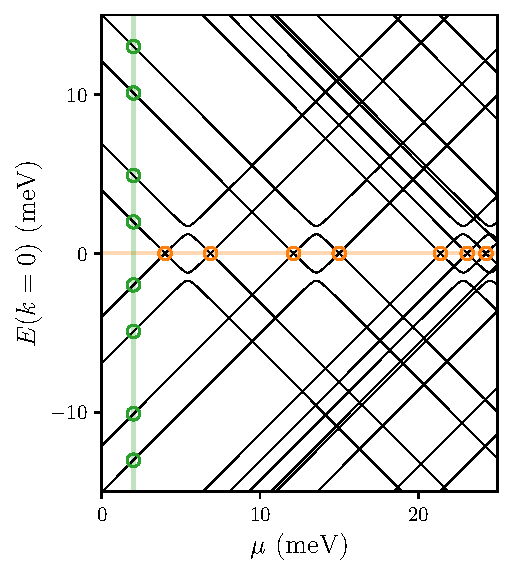
\includegraphics{chapter_introduction/figures/generalized_ev_problem.pdf}
\caption{Energy spectrum at $k=0$ of as a function of chemical potential $\mu$.
The orange circles are the real eigenvalues of Eq.~\eqref{eq:mu_ev_problem} lying at $E=0$ (the orange line).
The green circles are the solutions of $H_\textrm{BdG} \psi = E \psi$ at fixed $\mu$ marked by the green line.
To find the phase transitions with the latter approach, one needs to sweep over $\mu$ and find $E(k=0) < \epsilon$, where $\epsilon$ is the precision.
Using the generalized eigenvalue problem, we find all phase transitions at once.
\label{fig:mu_ev_problem}}
\end{center}
\end{figure}


% https://docs.lib.purdue.edu/cgi/viewcontent.cgi?article=1202&context=nanopub
% http://edu.itp.phys.ethz.ch/fs14/sst/Lecture-Notes.pdf

\subsection{Limits}
\co{Works only for systems with limited interaction, tightly bound electrons, large number of electrons, perfect lattice structure}
What it does not include.

\subsection{Complexity}
Still three dimensional systems are prohibitivly computationally expensive.


%%%%%%%%%%%%%%%%%%%%%%%%%%%%%%%%%%%%%%%%%%%%%%%%%%%%%%%%%%%%%%%%%%%%%%%%%%%%%%%%%%%%%%%
%%%%%%%%%%%%%%%%%%%%%%%%%%%%%% STRUCTURE OF THIS THESIS %%%%%%%%%%%%%%%%%%%%%%%%%%%%%%%
%%%%%%%%%%%%%%%%%%%%%%%%%%%%%%%%%%%%%%%%%%%%%%%%%%%%%%%%%%%%%%%%%%%%%%%%%%%%%%%%%%%%%%%


\section{Structure of this thesis}

Here, we give a brief overview of the topics explored in the following chapters.
\vspace{1mm}

\subsection{Chapter~\ref{ch:orbitalfield}: Orbital effect of magnetic field on the Majorana phase diagram}
Studies of Majorana bound states in semiconducting nanowires frequently neglect the orbital effect of a magnetic field.
Systematically studying its role leads us to several conclusions for designing Majoranas in this system.
Specifically, we show that for experimentally relevant parameter values the orbital effect of a magnetic field has a stronger impact on the dispersion relation than the Zeeman effect.
While Majoranas do not require the presence of only one dispersion subband, we observe that the size of the Majoranas becomes unpractically large, and the band gap unpractically small when more than one subband is filled.
Since the orbital effect of a magnetic field breaks several symmetries of the Hamiltonian, it leads to the appearance of large regions in parameter space with no band gap whenever the magnetic field is not aligned with the wire axis.
The reflection symmetry of the Hamiltonian with respect to the plane perpendicular to the wire axis guarantees that the wire stays gapped in the topologically nontrivial region as long as the field is aligned with the wire.
\vspace{1mm}

\subsection{Chapter~\ref{ch:supercurrent}: Supercurrent Interference in Few-Mode Nanowire Josephson Junctions}
Junctions created by coupling two superconductors via a semiconductor nanowire in the presence of high magnetic fields are the basis for the potential detection, fusion and braiding of Majorana bound states.
We study NbTiN/InSb nanowire/NbTiN Josephson junctions and find that the dependence of the critical current on the magnetic field exhibits gate-tunable nodes.
This is in contrast with a well-known Fraunhofer effect, under which critical current nodes form a regular pattern with a period fixed by the junction area.
Based on a realistic numerical model we conclude that the Zeeman effect induced by the magnetic field and the spin-orbit interaction in the nanowire are insufficient to explain the observed evolution of the Josephson effect.
We find the interference between the few occupied one-dimensional modes in the nanowire to be the dominant mechanism responsible for the critical current behavior.
We also report a strong suppression of critical currents at finite magnetic fields that should be taken into account when designing circuits based on Majorana bound states.
\vspace{1mm}

\subsection{Chapter~\ref{ch:spinorbit}: Spin-Orbit Protection of Induced Superconductivity in Majorana Nanowires}
Spin-orbit interaction (SOI) plays a key role in creating Majorana zero modes in semiconductor nanowires proximity coupled to a superconductor.
We track the evolution of the induced superconducting gap in InSb nanowires coupled to a NbTiN superconductor in a large range of magnetic field strengths and orientations.
Based on realistic simulations of our devices, we reveal SOI with a strength of 0.15--0.35 eV\AA.
Our approach identifies the direction of the spin-orbit field, which is strongly affected by the superconductor geometry and electrostatic gates.
\vspace{1mm}

\subsection{Chapter~\ref{ch:zigzag}: Title here for zigzag}
Abstract here for zigzag  % XXX: add this!
\vspace{1mm}

\subsection{Chapter~\ref{ch:shortjunction}: Robustness of Majorana bound states in the short-junction limit}
We study the effects of strong coupling between a superconductor and a semiconductor nanowire on the creation of the Majorana bound states, when the quasiparticle dwell time in the normal part of the nanowire is much shorter than the inverse superconducting gap.
This ``short-junction'' limit is relevant for the recent experiments using the epitaxially grown aluminum characterized by a transparent interface with the semiconductor and a small superconducting gap.
We find that the small superconducting gap does not have a strong detrimental effect on the Majorana properties.
Specifically, both the critical magnetic field required for creating a topological phase and the size of the Majorana bound states are independent of the superconducting gap.
The critical magnetic field scales with the wire cross-section, while the relative importance of the orbital and Zeeman effects of the magnetic field is controlled by the material parameters only: $g$ factor, effective electron mass, and the semiconductor-superconductor interface transparency.

\subsection{Chapter~\ref{ch:adaptive}: Title here for adaptive}
Abstract here for adaptive  % XXX: add this!
\vspace{1mm}

\references{dissertation}
